%%%%%%%%%%%%%%%%%%%%%%%%%%%%%%%%%%%%%%%%%%%%%%%%%%%%%%%%%%%%%%%%%%%%%%%%%%%%%%%%
%%%%%%%%%%%%%%%%%%%%%%%%%%%%%%%%%%%%%%%%%%%%%%%%%%%%%%%%%%%%%%%%%%%%%%%%%%%%%%%%
%
% A general frame for lecture slides and lecture notes in one file
% using LaTeX beamer
%
%%%%%%%%%%%%%%%%%%%%%%%%%%%%%%%%%%%%%%%%%%%%%%%%%%%%%%%%%%%%%%%%%%%%%%%%%%%%%%%%
%%%%%%%%%%%%%%%%%%%%%%%%%%%%%%%%%%%%%%%%%%%%%%%%%%%%%%%%%%%%%%%%%%%%%%%%%%%%%%%%
\documentclass[ignorenonframetext,11pt]{beamer}
%\usepackage[ngerman]{babel}
%\usepackage[T1]{fontenc}
\usepackage[utf8]{inputenc}
\usepackage{lmodern}
\usepackage{tcolorbox}
\usepackage{amsmath,amssymb,amsfonts}


% only presentation
\mode<presentation>
{
  \usetheme{default}
%  \usecolortheme{crane}
  \setbeamercovered{transparent}
%  \setlength{\parindent}{0pt}
%  \setlength{\parskip}{1.35ex plus 0.5ex minus 0.3ex}
%  \usefonttheme{structuresmallcapsserif}
  \usefonttheme{structurebold}
  \setbeamertemplate{theorems}[numbered]
  \setbeamertemplate{sidebar right}{}
  \usepackage{amscd}
}

% all after
\usepackage{tikz}
\usepackage{pgfplots,adjustbox}
\usepackage{eurosym}
\usepackage{graphicx}
\graphicspath{{.}{figures/}} 
\usepackage{multimedia}
\usepackage{psfrag}
\usepackage{listings}
% \lstset{language=C++, basicstyle=\ttfamily,
%   keywordstyle=\color{black}\bfseries, tabsize=4, stringstyle=\ttfamily,
%   commentstyle=\it, extendedchars=true, escapeinside={/*@}{@*/}}
\lstset{language=C++, basicstyle=\small\ttfamily,
  keywordstyle=\bfseries, tabsize=4, stringstyle=\ttfamily,morekeywords={decltype},
  commentstyle=\itshape, extendedchars=true, escapeinside={/*@}{@*/}}
\definecolor{darkgray}{gray}{0.4}
\lstset{keywordstyle=\color{violet},
  commentstyle=\color{darkgray},
  stringstyle=\color{orange},
  emph={bool,int,unsigned,char,true,false,void}, emphstyle=\color{blue},
  emph={[2]\#include,\#define,\#ifdef,\#endif}, emphstyle={[2]\color{violet}},
  emph={[3]Dune,Grid,SomeGrid,TheGrid,LeafIterator,LevelIterator,LeafIntersectionIterator,LevelIntersectionIterator,Geometry,Entity,EntityPointer,Codim,FieldVector,FieldMatrix}, emphstyle={[3]\color{blue}}
}
\usepackage{curves}
%\usepackage{epic}
\usepackage{calc}
%\usepackage{picinpar}
%\usepackage{fancybox}
%\usepackage{xspace}
\usepackage{enumerate}
\usepackage{algpseudocode}
\usepackage{color}
\usepackage{bold-extra}
\usepackage{bm}
\usepackage{stmaryrd}
%\usepackage[squaren]{SIunits}
\usepackage{nicefrac}

\usepackage{fancyvrb,bbm,xspace}
\usepackage{lmodern}
\usepackage{fancyvrb,bbm,xspace}
\usepackage[binary-units]{siunitx}
\usepackage{xcolor,tabu}

\definecolor{niceblue}{rgb}{0.122,0.396,0.651}   %% 31, 101, 166 or #1F65A6
\definecolor{niceorange}{RGB}{255,205,86}        %% #FFCD56
\definecolor{nicered}{RGB}{220,20,60}                      %% rgb(220, 20, 60)
\definecolor{niceteal}{HTML}{00A9AB}
\definecolor{niceviolet}{HTML}{820080}

\definecolor{niceblueLight}{HTML}{91CAFB}
\definecolor{niceblueVeryLight}{HTML}{DDEFFF}

\usepackage{dsfont}

\mode<presentation>
{
\theoremstyle{definition}
}
% \newtheorem{Def}{Definition}%[section]
% \newtheorem{Exm}[Def]{Example}
% \newtheorem{Lem}[Def]{Lemma}
% \newtheorem{Rem}[Def]{Remark}
% \newtheorem{Rul}[Def]{Rule}
% \newtheorem{Thm}[Def]{Theorem}
% \newtheorem{Cor}[Def]{Corollary}
% \newtheorem{Obs}[Def]{Observation}
% \newtheorem{Ass}[Def]{Assumption}
% \newtheorem{Pro}[Def]{Property}
% \newtheorem{Alg}[Def]{Algorithm}
% \newtheorem{Prp}[Def]{Proposition}
% \newtheorem{Lst}[Def]{Listing}

\newenvironment{codebox}{%
  \begin{tcolorbox}[size=small,oversize,boxrule=0pt,colframe=white]}{%
  \end{tcolorbox}}
\newenvironment{cppcode}[1]
   {\begin{coebox}%
    \begin{lstlisting}[basicstyle=\scriptsize\ttfamily]}
  {\end{lstlisting}\end{codebox}}
\newcommand{\rightarrownice}{\tikz{%
    \draw[-latex,line width=2pt, color=structure.fg]   (0pt,0pt) -- +(2em,0) node[thin,right] {};}}

% math symbols
\newcommand{\C}{\mathbb{C}}
\newcommand{\R}{\mathbb{R}}
\newcommand{\N}{\mathbb{N}}
\newcommand{\Z}{\mathbb{Z}}
\newcommand{\Q}{\mathbb{Q}}
\newcommand{\K}{\mathbb{K}}
\newcommand{\blue}{\color[rgb]{0,0,1}}
\newcommand{\green}{\color[rgb]{0,1,0}}
\newcommand{\red}{\color[rgb]{1,0,0}}
\newcommand{\violet}{\color[rgb]{1,0,1}}
\newcommand{\uu}{\mathbf{u}}
\newcommand{\nn}{\mathbf{n}}
\newcommand{\diffd}{\,d}

% Delete this, if you do not want the table of contents to pop up at
% the beginning of each subsection:
\AtBeginSection[]
{
  \begin{frame}<beamer>
    \frametitle{Contents}
    \tableofcontents[sectionstyle=show/shaded,subsectionstyle=hide/hide/hide]
%\tableofcontents[currentsection]
  \end{frame}
}

% Title definition
\title{The DUNE Grid Interface\\An Introduction}
\author{Christian Engwer}
\institute[]
{
  Applied Mathematics, WWU Münster\\
  Orleans-Ring 10, 48149 Münster
}
\date{March 7, 2017}

%%%%%%%%%%%%%%%%%%%%%%%%%%%%%%%%%%%%%%%%%%%%%%%%%%%%%%%%%%%%%%%%%%%%%%%%%%%%%%%%
%%%%%%%%%%%%%%%%%%%%%%%%%%%%%%%%%%%%%%%%%%%%%%%%%%%%%%%%%%%%%%%%%%%%%%%%%%%%%%%%
%
% now comes the individual stuff lecture by lecture
%
%%%%%%%%%%%%%%%%%%%%%%%%%%%%%%%%%%%%%%%%%%%%%%%%%%%%%%%%%%%%%%%%%%%%%%%%%%%%%%%%
%%%%%%%%%%%%%%%%%%%%%%%%%%%%%%%%%%%%%%%%%%%%%%%%%%%%%%%%%%%%%%%%%%%%%%%%%%%%%%%%

\begin{document}

\begin{frame}
  \titlepage
  \uncover<2->{
  \begin{quote}
    People think that computer science is the art of geniuses but the
    actual reality is the opposite, just many people doing things that
    build on each other, like a wall of mini stones.
    
    \hfill--- Donald E. Knuth
  \end{quote}}
\end{frame}

\begin{frame}
  \frametitle{Why Grids?}
  Weak formulation of boundary value problem:\\
  \begin{equation*}
    \text{Find $u \in U$ s.t.}\qquad
    a(u,v) = l(v) \quad \forall\,v \in V.
  \end{equation*}
  $a(u,v)$ and $l(v)$ are (bi)linear forms, e.g.
  \begin{equation*}
    a(u,v) = \int_\Omega \nabla u \cdot \nabla v \diffd x,
  \end{equation*}
  \raisebox{2ex}{with spatial domain $\Omega \subset \R^d$.}
  \pause
  \begin{center}
    \structure{How to evaluate the integrals?}
  \end{center}
  
  \begin{itemize}
  \item No analytic integrals available for $a(u,v)$ and $l(v)$.
  \item No analytic description for the shape of $\Omega \subset \R^d$.
  \end{itemize}
\pause
\begin{center}
  \rightarrownice Use a numerical quadrature scheme!
\end{center}
\end{frame}


\begin{frame}
  \frametitle{Numerical Quadrature}
  \begin{itemize}
  \item Approximate integral by a weighted sum of function evaluations at sampling points:
  \begin{equation*}
    \int_\Omega f(x) \diffd x \approx \sum_{i = 1}^N w_i f(x_i)
  \end{equation*}
  with weights $w_i$ and sampling points $x_i$, $i = 1,\dots,N$.\\[1em]
\item Different construction methods for $w_i$ and $x_i$
  \begin{itemize}
  \item Typically uses series of polynomials (Legendre, Lagrange, Lobatto, \dots).
  \item Exact for polynomial $f$ up to a predefined order.
  \end{itemize}
\item Quadrature scheme depends on $\Omega$!
  \begin{itemize}
  \item Most schemes only available for simple shapes (triangle, square, tetrahedron, \dots).
  \item Quadrature on complicated shapes done by approximating $\Omega$ by small volumes of regular shape.
  \end{itemize}
  \end{itemize}
\end{frame}


\begin{frame}
  \frametitle{Computational Grid}
  \begin{columns}
    \begin{column}{0.3\textwidth}
      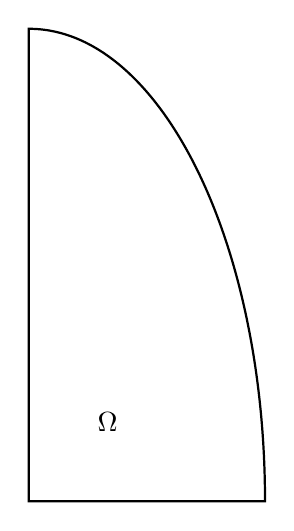
\begin{tikzpicture}
        \draw[thick]
        (0,0) -- (3,0) arc[start angle=0, end angle=90, x radius=3, y radius=6] -- cycle;
        \node at (1,1) {$\Omega$};
      \end{tikzpicture}
    \end{column}
    \begin{column}{0.3\textwidth}
      \includegraphics[width=3cm]{ellipsemeshcoarse-cropped}
    \end{column}
    \begin{column}{0.3\textwidth}
      \includegraphics[width=3cm]{ellipsemesh-cropped}
    \end{column}
  \end{columns}
\end{frame}

\begin{frame} \frametitle{The DUNE Grid Module}
  \begin{itemize}
  \item The DUNE Grid Module is one of the five DUNE Core Modules.

  \item DUNE wants to provide an interfaces for grid-based
    methods. Therefore the concept of a \emph{Grid} is the central part
    of DUNE.

  \item \texttt{dune-grid} provides the interfaces, following the concept
    of a \emph{Grid}.

  \item Is implementation follows the three \emph{design principles} of
    DUNE:
    \begin{description}[~~~Legacy Code:]
    \item[Flexibility:]
      \onslide<0->{Separation of data structures and algorithms.}
    \item[Efficiency:]
      \onslide<0->{Generic programming techniques.}
    \item[Legacy Code:]
      \onslide<0->{Reuse existing finite element software.}
    \end{description}

  \end{itemize}
\end{frame}

\begin{frame}
  \frametitle<presentation>{Designed to support a wide range of Grids}
  \frametitle<article>{DUNE is designed to support a wide range of Grids:}
  \only<article>{\vspace*{2ex}}
  \includegraphics[width=\linewidth]{grids}
\end{frame}

\begin{frame}
\frametitle{DUNE Grid Interface\footnote{\tiny Bastian,
Blatt, Dedner, Engwer, Kl{\"{o}}fkorn, Kornhuber,
Ohlberger, Sander: {\em A generic grid interface for parallel and adaptive
  scientific computing. Part {I}: Implementation and tests in {DUNE}}.
  Computing, 82(2-3):121--138, 2008.} Features}
\begin{itemize}
\item Provide abstract interface to grids with:
\begin{itemize}
\item Arbitrary dimension embedded in a world dimension,
\item multiple element types,
\item conforming or nonconforming,
\item hierarchical, local refinement,
\item arbitrary refinement rules (conforming or nonconforming),
\item parallel data distribution and communication,
\item dynamic load balancing.
\end{itemize}
\item Reuse existing implementations (ALU, UG, Alberta) + special
implementations (YaspGrid, FoamGrid).
\item Meta-Grids built on-top of the interface (GeometryGrid, SubGrid,
  MultiDomainGrid)
\end{itemize}
\end{frame}

\section{The Grid}

\begin{frame}
  \frametitle{The Grid}
  \emph{A formal specification of grids is required to enable an
  accurate description of the grid interface.}
  \only<presentation>{\vspace*{5mm}}
  \begin{columns}
    \begin{column}{0.33\linewidth}
      \only<presentation>{
      \includegraphics[width=0.9\linewidth]{hierref}\\
      \centerline{\tiny Hierarchic Grid}}
    \end{column}\hfill
    \begin{column}{0.6\linewidth}
      In DUNE a \emph{Grid} is always a hierarchic grid of dimension
      $d$, existing in a $w$ dimensional
      space. \only<presentation>{\par}
      The Grid is parametrised by
      \begin{itemize}
      \item the dimension $d$,
      \item the world dimension $w$
      \item and the maximum level $J$.
      \end{itemize}
    \end{column}
  \end{columns}
  \only<article>{
    \begin{center}
      \includegraphics[width=0.5\linewidth]{hierref}\\
      \tiny Hierarchic Grid
    \end{center}
  }
  \pause
  \only<presentation>{\vspace*{5mm}
  \emph{Within todays excercises we will always assume $d=w$ and we will
    ignore the hierarchic structure of the grids we deal with.}}
\end{frame}

\begin{frame} \frametitle{The Grid\ldots A Container of Entities\ldots}

  In the DUNE sense a \emph{Grid} is a container of entities:

  \only<presentation>{\vspace*{5mm}}
  \begin{columns}
    \begin{column}{5mm}
    \end{column}
    \begin{column}{0.5\linewidth-5mm}
      \begin{onlyenv}<presentation>
        \includegraphics<1-2>[width=\linewidth]{entities}
        \includegraphics<3->[width=\linewidth]{entities_cd}
      \end{onlyenv}
      \begin{onlyenv}<article>
        \vspace*{2ex}
        ~\hfill\includegraphics[width=0.4\linewidth]{entities}\hfill
        \includegraphics[width=0.4\linewidth]{entities_cd}\hfill~
      \end{onlyenv}
    \end{column}\hfill
    \begin{column}{0.5\linewidth}
      \begin{itemize}
      \item vertices \only<3->{\emph{(Entity codim = $d$)}},
      \item edges \only<3->{\emph{(Entity codim = $d-1$)}},
      \item faces \only<3->{\emph{(Entity codim = $1$)}},
      \item cells \only<3->{\emph{(Entity codim = $0$)}}, \ldots{}
      \end{itemize}
    \end{column}
  \end{columns}
  \only<presentation>{\vspace*{5mm}}

  \pause{In order to do dimension independent programming, we need a
    dimension independent naming for different entities.}
  \only<presentation>{\par}
  \pause{We distinguish entities according to their codimension.}
  \only<presentation>{\par}
  Entities of codim = $c$ contain subentities of codim = $c+1$. This
  gives a recursive construction down to codim = $d$.

\end{frame}

\begin{frame}[fragile,fragile] \frametitle{The DUNE Grid Interface}
  The DUNE Grid Interface is a collection of classes and methods

  \only<presentation>{\vfill}
\begin{codebox}
\begin{lstlisting}[basicstyle=\scriptsize\ttfamily]
#include <dune/grid/yaspgrid.hh>

...

using Grid = Dune::YaspGrid<2>;
Grid grid({4,4},{1.0,1.0},{false,false});
auto gv = grid.leafGridView();
for (const auto& cell : elements(gv)) {
  // do something
}
\end{lstlisting}
\end{codebox}

  \only<presentation>{\vfill}
  %The grid will provide typedefs for all these classes.

  \pause
  \only<presentation>{\vfill}
  \emph{We will now get to know the most important classes and see how they
  interact.}
\end{frame}

\end{document}

\begin{frame} \frametitle{Modifying a Grid}
  The DUNE Grid interface follows the \emph{View-only} Concept.
  \pause
  \only<presentation>{\vfill}
  \structure{View-Only Concept}
  \begin{itemize}
  \item Views offer (read-only) access to the data
    \begin{itemize}
    \item Read-only access to grid entities allow the consequent use of
      \cpp!const!.
    \item Access to entities is only through iterators for a
      certain view.
      \begin{itemize}
      \item[\rightarrownice] \emph{This allows on-the-fly implementations.}
      \end{itemize}
    \end{itemize}
  \item  Data can only be modified in the primary container \emph{(the Grid)}
  \end{itemize}
  \pause
  \only<presentation>{\vfill}
  \structure{Modification Methods:}
  \begin{itemize}
  \item  Global Refinement

  \item  Local Refinement \& Adaption

  \item  Load Balancing
  \end{itemize}
\end{frame}

\section{Views to the Grid}

\begin{frame} \frametitle{Views to the Grid}

  A Grid offers two major views:

  \only<presentation>{\vspace*{5mm}}
  \begin{columns}
    \begin{column}{0.5\linewidth}
      \begin{onlyenv}<presentation>
        \includegraphics<1-2>[width=\linewidth]{views}
        \includegraphics<3->[width=\linewidth]{views2}
      \end{onlyenv}
      \begin{onlyenv}<article>
        \begin{center}
          \includegraphics[width=0.7\linewidth]{views2}
        \end{center}
      \end{onlyenv}
    \end{column}
    \begin{column}{0.5\linewidth}
      \structure{levelwise:}\\
      \only<presentation>{\small}
      all entities associated with the same level.\\
      \uncover<2->{
        \emph{Note: not all levels must cover the whole domain.}}

      \only<presentation>{\vspace*{5mm}}
      \normalsize
      \structure{leafwise:}\\
      \only<presentation>{\small}
      all leaf entities (entities which are not refined).\\
      \uncover<3->{
        The leaf view can be seen as the projection of a
        levels onto a flat grid. It again covers the whole domain.}
    \end{column}
  \end{columns}

\end{frame}

\begin{frame} \frametitle{Views to the Grid}
  \framesubtitle{Dune::GridView}

  \begin{itemize}
  \item The \cpp!Dune::GridView!  class consolidates all
    information depending on the current View.
    \pause
  \item Every Grid must provide
    \begin{itemize}
    \item \cpp!Grid::LeafGridView! and
    \item \cpp!Grid::LevelGridView!.
    \end{itemize}
    \pause

  \item The \cpp!Grid! creates a new view every time you ask it for one, so you need
    to store a copy of it.
  \item Accessing the Views:
    \begin{itemize}
    \item \cpp!Grid::leafGridView()! and
    \item \cpp!Grid::levelGridView(int level)!.
    \end{itemize}
  \end{itemize}
\end{frame}

\begin{frame}[fragile]
  \frametitle{Iterating over grid entities}
Typically, most code uses the grid to iterate over some of its entities (e.g.\ cells) and perform
some calculations with each of those entities.
\begin{itemize}
\item \cpp!GridView! supports iteration over all entities of one codimension.
\item Iteration uses C++11 range-based for loops:
  \begin{cppcode}
    for (const auto& cell : elements(gv)) {
      // do some work with cell
    }
  \end{cppcode}
\item The type in front of \cpp!cell! is important:
  \begin{itemize}
  \item If you create an entity in a range-based for loop, use \cpp!const auto&!.
  \item In \emph{all} other cases, use plain \cpp!auto!!
  \end{itemize}
  If you do not follow this advice, your program may crash in unpredictable ways.
\end{itemize}
\end{frame}


\begin{frame}[fragile]
  \frametitle{Iteration functions}
  \begin{cppcode}
    for (const auto& cell : elements(gv)) {
      // do some work with cell
    }
  \end{cppcode}
  Depending on the entities you are interested in, you can use one of the following functions:
  \begin{cppcode}
    // Iterates over cells   (codim = 0)
    for (const auto& c : elements(gv))
    // Iterates over vertices  (dim = 0)
    for (const auto& v : vertices(gv))
    // Iterates over facets  (codim = 1)
    for (const auto& f : facets(gv))
    // Iterates over edges     (dim = 1)
    for (const auto& e : edges(gv))

    // Iterates over entities with a given codimension (here: 2)
    for (const auto& e : entities(gv,Dune::Codim<2>{}))
    // Iterates over entities with a given dimension (here: 3)
    for (const auto& e : entities(gv,Dune::Dim<2>{}))
  \end{cppcode}
\end{frame}

% \begin{frame}
%   \frametitle{LevelGridView versus LeafGridView}
%   \begin{columns}
%     \begin{column}{0.47\linewidth}
%       \begin{center}
%         \begin{onlyenv}<article>
%           \includegraphics[width=0.7\linewidth]{iterators}
%         \end{onlyenv}
%       \end{center}
%       \begin{onlyenv}<presentation>
%         \includegraphics[width=\linewidth]{iterators}
%       \end{onlyenv}
%     \end{column}
%     \begin{column}{0.53\linewidth}
%     \end{column}
%   \end{columns}
% \end{frame}


\section{Entities}

\begin{frame}[fragile] \frametitle{Entities}

  \structure{Iterating over a grid view, we get access to the entities.}

  \begin{cppcode}
    for (const auto& cell : elements(gv)) {
      cell.?????(); // what can we do here?
    }
  \end{cppcode}

  \pause
  \begin{itemize}
  \item Entities cannot be modified.
  \item Entities can be copied and stored\\(but copies might be expensive!).
    \pause
  \item Entities provide topological and geometrical information.
  \end{itemize}
\end{frame}

\begin{frame}
  \frametitle{Entities}

  \structure{An Entity $E$ provides both topological information}
  \begin{itemize}
  \item Type of the entity (triangle, quadrilateral, etc.).
  \item Relations to other entities.
  \end{itemize}
  \structure{and geometrical information}
  \begin{itemize}
  \item Position of the entity in the grid.
  \end{itemize}

  \only<presentation>{\vfill}
  \pause
  \begin{columns}
    \begin{column}{5mm}
    \end{column}
    \begin{column}{0.4\textwidth}
      \begin{center}
        \visible<presentation|2->{
          \includegraphics[width=\linewidth]{refelem-mapping}}\\
        \begin{onlyenv}<article>
          \includegraphics[width=0.6\linewidth]{refelem-mapping}\\
        \end{onlyenv}
        \centerline{\tiny Mapping from $\hat{\Omega}$ into global coordinates.}
      \end{center}
    \end{column}
    \begin{column}{0.5\textwidth}
      \structure{Entity $E$ is defined by\dots{}}
        \begin{itemize}
        \item Reference Element $\hat{\Omega}$
        \item Transformation $T_E$
        \end{itemize}
    \end{column}
  \end{columns}

  \only<presentation>{\vfill}
  \pause
  \cpp!GridView::Codim<c>::Entity!
  implements the entity concept.

\end{frame}

\begin{frame}[fragile]
  \frametitle{Storing Entities}

  \vfill

  \pause
  \cpp!GridView::Codim<c>::Entity!
  \begin{itemize}
  \item Entities can be copied and stored like any normal object.
  \item Important: There can be \emph{multiple} entity objects for a single logical grid entity (because they can be copied)
  \item \emph{Memory expensive, but fast.}
  \end{itemize}

  \vfill

  \pause

  \cpp!GridView::Codim<c>::EntitySeed!


  \begin{itemize}
  \item Store minimal information to find an entity again.
  \item Create like this:
    \begin{cppcode}
      auto entity_seed = entity.seed();
    \end{cppcode}
  \item The grid can create a new \cpp!Entity! object from an \cpp!EntitySeed!:
    \begin{cppcode}
      auto entity = grid.entity(entity_seed);
    \end{cppcode}
  \item \emph{Memory efficient, but run-time overhead to recreate entity.}
  \end{itemize}

\end{frame}

% \only<article>{\newpage}

\subsection{Reference Elements}
\begin{frame} \frametitle{Reference Elements}

  \begin{description}
  \item[\tt Dune::GeometryType] identifies the type of the
    entities Referenceelement.\only<presentation>{\\}
    It bundles a \emph{topology ID} and the dimension.
  \item[\tt Grid::Codim<c>::Entity::type()] \only<presentation>{~\\}
    returns the GeometryType of the entity.
  \end{description}

  \begin{onlyenv}<presentation>
    ~\hfill\includegraphics[width=0.24\linewidth]{gg_triangle}
    \hfill\includegraphics[width=0.28\linewidth]{gg_hexahedron}
    \hfill\includegraphics[width=0.22\linewidth]{gg_prism}
    \hfill~

    ~\hfill\parbox{0.24\linewidth}{\centering simplex 2D}
    \hfill\parbox{0.28\linewidth}{\centering cube 3D}
    \hfill\parbox{0.22\linewidth}{\centering prism} \hfill~
  \end{onlyenv}
  \begin{onlyenv}<article>
    \textbf{1D}:
    \begin{center}
      \includegraphics[width=0.23\linewidth]{gg_line}

      line 1D (both simplex 1D \& cube 1D)
    \end{center}
    \textbf{2D:}
    \begin{center}
      \begin{tabular}{cccc}
        \includegraphics[height=0.23\linewidth]{gg_triangle} &
        \includegraphics[height=0.23\linewidth]{gg_quadrilateral}\\
        simplex 2D & cube 2D\\
      \end{tabular}
    \end{center}
    \textbf{3D:}
    \begin{center}
      \begin{tabular}{cccc}
        \includegraphics[height=0.23\linewidth]{gg_tetrahedron} &
        \includegraphics[height=0.23\linewidth]{gg_tetrahedron_edges} &
        \includegraphics[height=0.23\linewidth]{gg_hexahedron} &
        \includegraphics[height=0.23\linewidth]{gg_hexahedron_edges}
        \\
        simplex 3D (faces) & simplex 3D (edges) & cube 3D (faces) & cube 3D (edges)\\

      \end{tabular}
    \end{center}
    \begin{center}
      \begin{tabular}{cccc}
        \includegraphics[height=0.23\linewidth]{gg_prism} &
        \includegraphics[height=0.23\linewidth]{gg_prism_edges} &
        \includegraphics[height=0.23\linewidth]{gg_pyramid} &
        \includegraphics[height=0.23\linewidth]{gg_pyramid_edges}
        \\
        prism (faces) & prism (edges) & pyramid (faces) & pyramid (edges)\\
      \end{tabular}
    \end{center}
    For more information see the documentation on reference elements
    (\url{http://www.dune-project.org/doc-2.3.0/doxygen/html/group__GeometryReferenceElements.html})
  \end{onlyenv}
\end{frame}

%\only<article>{\newpage}


\subsection{Geometry}

\begin{frame}
  \frametitle{Geometry}

  Transformation $T_E$
  \begin{itemize}
  \item Maps from one space to an other.
  \item Main purpose is to map from the reference element to global coordinates.
  \item Provides transposed inverse of the Jacobian ($J^{-T}(T_E)$).
  \end{itemize}

  \visible<presentation|1->{
    \begin{center}
    \includegraphics[width=0.5\linewidth]{refelem-mapping}\end{center}}


 %  \only<presentation>{\vfill}
 %  \pause
 %  \lstinline!Grid::Codim<c>::Geometry!
 %  provides this data:

 %  \only<presentation>{\vfill}
 %  \pause

 %  \begin{center}
 %    \begin{tabular}{l|l\amode{|p{8cm}}{}}
 %      \hline
 %      Method name & Parameter \amode{& Result}{} \\\hline
 %      \lstinline[basicstyle=\scriptsize\ttfamily]!global! & local coordinate
 %      \amode{& transform from reference (local) coordinate
 %        system to target (global) coordinate system}{}\\
 %      \lstinline[basicstyle=\scriptsize\ttfamily]!local! & global coordinate
 %      \amode{& transform from target (global) coordinate
 %        system to reference (local) coordinate system}{}\\
 %      \lstinline[basicstyle=\scriptsize\ttfamily]!center! & none
 %      \amode{& center of entity in target (global) coordinates}{}\\
 %      \lstinline[basicstyle=\scriptsize\ttfamily]!volume! & none
 %      \amode{& volume of entity in units of the target (global)
 %        coordinate system}{}\\
 %      \lstinline[basicstyle=\scriptsize\ttfamily]!integrationElement! & local coordinate
 %      \amode{& Determinant of the jacobian of the
 %        Transformation from local to global coordinates. For affine
 %        transformations this is the volume}{}\\
 %      \lstinline[basicstyle=\scriptsize\ttfamily]!jacobianInverseTransposed! & local coordinate
 %      \amode{& the inverse of the transposed jacobian of the
 %        transformation; this is necessary to correctly transform
 %        gradients from local to global coordinates}{}
 %      \\\hline
 %    \end{tabular}
 % \end{center}
\end{frame}


\begin{frame}[fragile]
  \frametitle{Geometry II}
  \begin{itemize}
  \item Obtain Geometry from entity
    \begin{cppcode}
      auto geo = entity.geometry();
    \end{cppcode}
  \item Convert local coordinate to global coordinate
    \begin{cppcode}
      auto x_global = geo.global(x_local);
    \end{cppcode}
  \item Convert global coordinate to local coordinate
    \begin{cppcode}
      auto x_local = geo.local(x_global);
    \end{cppcode}
  \end{itemize}
\end{frame}


\begin{frame}[fragile]
  \begin{itemize}
  \item Get center of geometry in global coordinates
    \begin{cppcode}
      auto center = geo.center();
    \end{cppcode}
  \item Get number of corners of the geometry (e.g. 3 for a triangle)
    \begin{cppcode}
      auto num_corners = geo.corners();
    \end{cppcode}
  \item Get global coordinates of $i$-th geometry corner ($0 \leq i < \cpp!geo.corners()!$)
    \begin{cppcode}
      auto corner_global = geo.corner(i);
    \end{cppcode}
  \end{itemize}
\end{frame}


\begin{frame}[fragile]
  \begin{itemize}
  \item Get type of reference element
    \begin{cppcode}
      auto geometry_type = geo.type(); // e.g. square, triangle, ...
    \end{cppcode}
  \item Find out whether geometry is affine
    \begin{cppcode}
      if (geo.affine()) {
        // do something optimized
      }
    \end{cppcode}
  \item Get volume of geometry in global coordinate system
    \begin{cppcode}
      auto volume = geo.volume();
    \end{cppcode}
  \item Get integration element for a local coordinate (required for numerical integration)
    \begin{cppcode}
      auto mu = geo.integrationElement(x_local);
    \end{cppcode}
  \end{itemize}
\end{frame}

\begin{frame}[fragile]
  \frametitle{Gradient Transformation}
  Assume
  \begin{equation*}
    f : \Omega \rightarrow \R
  \end{equation*}
 evaluated on a cell $E$, i.e.\ $f\bigl(T_E(\hat{x})bigr)$.\\[1em] The gradient of $f$ is then given by
 \begin{equation*}
   J_T^{-T}(\hat{x})\hat{\nabla}f\bigl(T_E(\hat{x})\bigr):
 \end{equation*}
  \begin{cppcode}
    auto x_global = geo.global(x_local);
    auto J_inv = geo.jacobianInverseTransposed(x_local);
    auto tmp = gradient(f)(x_global); // gradient(f) supplied by user
    auto gradient = tmp;
    J_inv.mv(tmp,gradient);
  \end{cppcode}
\end{frame}

\begin{frame}[fragile]
\frametitle{Example: Average of a function f on a GridView}
$\frac{1}{|\Omega|}\int_{\Omega}f(x) \diffd x \approx \frac{1}{\sum_{E \in GV} |e|}\sum_{E \in GV}\sum_{i \in QR} f(T_e(x_i)) w_i |\det J_E^T(x_i)|^{1/2}$
  \begin{cppcode}
    double value = 0.0, volume = 0.0;
    for (const auto& cell : elements(gv)) {
      auto geo = cell.geometry();
      // integrate with numerical quadrature
      for (auto& ip : Dune::QuadratureRules<double,2>::general(geo.type(),2)) {
        auto x_local = ip.position();
        auto x_global = geo.global(x_local);
        // accumulate integral contribution
        value += f(x_global) * ip.weight() * geo.integrationElement(x_local);
      }
      volume += geo.volume();
    }
    std::cout << "Average: " << value / volume << std::endl;
  \end{cppcode}
\end{frame}

%\only<article>{\newpage}


\subsection{Intersections}
\begin{frame}[fragile] \only<presentation>{\frametitle{Intersections}}

  \begin{columns}
    \begin{column}{0.75\linewidth}
      \begin{itemize}
      \item Grids may be non conforming.
      \item Entities can intersect with neighbours and boundary.
      \item Represented by \cpp!Intersection! objects.
      \item Intersections hold topological and
        geometrical information.
      \item Intersections depend on the view:
% TODO: Skizze?
      \item \textbf{Note:} Intersections are always of
        codimension 1!
      \end{itemize}
    \end{column}
    \begin{column}{0.25\linewidth}
      \begin{center}
        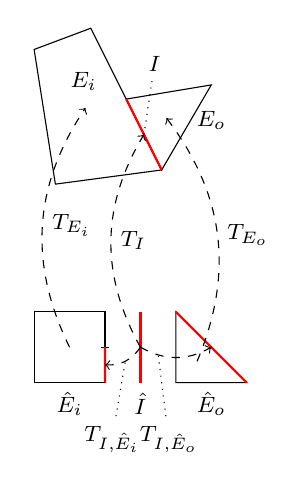
\begin{tikzpicture}[font=\footnotesize,scale=0.9]
\draw(2,0) -- (3,0) -- (2,1) -- cycle;

\draw[thick,red] (1.5,0) -- (1.5,1);

\draw (0,0) rectangle (1,1);

\draw (1.8,3) -- (1.3,4) -- (2.5,4.2) -- cycle;
\draw (1.8,3) -- (0.8,5) -- (0,4.7) -- (0.3,2.8) -- cycle;
\draw (0.95,0.5) -- (1.05,0.5);

\draw[thick,red]
  (1,0) -- (1,0.5)
  (2,1) -- (3,0)
  (1.8,3) -- (1.3,4);


\path
  (0.5,0.5) coordinate(e1r)
  (2.3,0.3) coordinate(e2r)
  (1.5,0.5) coordinate(ir)
  (0.725,3.875) coordinate(e1w)
  (1.867,3.733) coordinate(e2w)
  (1.55,3.5) coordinate(iw)
  (1,0.25) coordinate(ie1)
  (2.5,0.5) coordinate(ie2);

\draw[dashed]
  (ir)  edge[->,bend left]  node[right] {$T_I$}       (iw)
  (e1r) edge[->,bend left]  node[right] {$T_{E_i}$}   (e1w)
  (e2r) edge[->,bend right] node[right]  {$T_{E_o}$}   (e2w)
  (ir)  edge[->,bend left]  coordinate(ie1c)  (ie1)
  (ir)  edge[->,bend right] node(ie2c) [near start] {}  (ie2);

\node (ie1label) at(1.1,-0.8) {$T_{I,\hat{E}_i}$};
\node (ie2label) at(1.9,-0.8) {$T_{I,\hat{E}_o}$};
\node (ilabel) at (1.7,4.5) {$I$};

\draw[dotted]
  (ie1label) edge (ie1c)
  (ie2label) edge (ie2c.center)
  (ilabel) edge (iw);

\node at(1.5,-0.3) {$\hat{I}$};
\node at(0.5,-0.3) {$\hat{E}_i$};
\node at(2.5,-0.3) {$\hat{E}_o$};
\node at(0.7,4.25) {$E_i$};
\node at(2.5,3.7) {$E_o$};
        \end{tikzpicture}
      \end{center}
    \end{column}
  \end{columns}

\end{frame}

% \begin{frame} \frametitle{Intersection Interface}
%   Dereferencing \cpp!IntersectionIterator! yields \cpp!Intersection!:
%   \begin{columns}
%     \begin{column}{0.4\linewidth}
%       \begin{center}
%         \includegraphics<presentation>[width=\linewidth]{intersection}
%       \end{center}
%     \end{column}
%     \begin{column}{0.6\linewidth}
%     \scriptsize
%     \begin{tabular}{l\amode{|p{0.2\linewidth}}{}|p{0.3\linewidth}}
%       \hline
%       Method name & \amode{Parameter &}{} Result \\\hline
%       \lstinline[basicstyle=\scriptsize\ttfamily]!boundary! &
%       \amode{none &}{}
%       Boolean \\
%       \lstinline[basicstyle=\scriptsize\ttfamily]!neighbor! &
%       \amode{none &}{}
%       Boolean \\
%       \lstinline[basicstyle=\scriptsize\ttfamily]!inside! &
%       \amode{none &}{}
%       EntityPointer to $E$ \\
%       \lstinline[basicstyle=\scriptsize\ttfamily]!outside! &
%       \amode{none &}{}
%       EntityPointer to $E'$ \\
%       \lstinline[basicstyle=\scriptsize\ttfamily]!geometry! &
%       \amode{none &}{}
%       Geometry $T_{I}$ \\
%       \lstinline[basicstyle=\scriptsize\ttfamily]!geometryInInside! &
%       \amode{none &}{}
%       Geometry $T_{I,E}$ \\
%       \lstinline[basicstyle=\scriptsize\ttfamily]!geometryInOutside! &
%       \amode{none &}{}
%       Geometry $T_{I,E'}$ \\
%       \lstinline[basicstyle=\scriptsize\ttfamily]!unitOuterNormal! &
%       \amode{$\hat{I}$ local coordinate &}{}
%       outer normal $n$, $|n| = 1$\\
%       \lstinline[basicstyle=\scriptsize\ttfamily]!centerUnitOuterNormal! &
%       \amode{none &}{}
%       outer normal at \mbox{geometry().center()}
%       \\\hline
%     \end{tabular}
%     \end{column}
%   \end{columns}

% \end{frame}


\begin{frame}[fragile]
  \frametitle{Intersection Interface}
  \begin{itemize}
  \item Is this an intersection with the domain boundary?
    \begin{cppcode}
      bool b = intersection.boundary();
    \end{cppcode}
  \item Is there an entity on the outside of the intersection?
    \begin{cppcode}
      bool b = intersection.neighbor();
    \end{cppcode}
  \item Get the cell on the inside
    \begin{cppcode}
      auto inside_cell = intersection.inside();
    \end{cppcode}
  \item Get the cell on the outside
    \begin{cppcode}
      // Only do this if intersection.neighbor() == true
      auto outside_cell = intersection.outside();
    \end{cppcode}
  \end{itemize}

\end{frame}



\begin{frame}[fragile] \frametitle{Intersection: Geometries}
  \begin{columns}
    \begin{column}{0.75\linewidth}
      \begin{itemize}
      \item Get mapping from intersection reference element to global coordinates
        \begin{cppcode}
          auto world_geo = intersection.geometry();
        \end{cppcode}
      \item Get mapping from intersection reference element to reference element of inside cell
        \begin{cppcode}
          auto inside_geo = intersection.geometryInInside();
        \end{cppcode}
      \item Get mapping from intersection reference element to reference element of outside cell
        \begin{cppcode}
          auto outside_geo = intersection.geometryInOutside();
        \end{cppcode}
      \end{itemize}
    \end{column}
 \begin{column}{0.25\linewidth}
      \begin{center}
        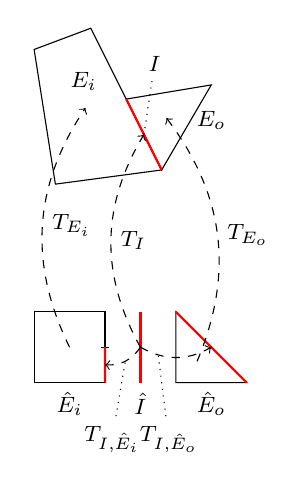
\begin{tikzpicture}[font=\footnotesize,scale=0.9]
\draw(2,0) -- (3,0) -- (2,1) -- cycle;

\draw[thick,red] (1.5,0) -- (1.5,1);

\draw (0,0) rectangle (1,1);

\draw (1.8,3) -- (1.3,4) -- (2.5,4.2) -- cycle;
\draw (1.8,3) -- (0.8,5) -- (0,4.7) -- (0.3,2.8) -- cycle;
\draw (0.95,0.5) -- (1.05,0.5);

\draw[thick,red]
  (1,0) -- (1,0.5)
  (2,1) -- (3,0)
  (1.8,3) -- (1.3,4);


\path
  (0.5,0.5) coordinate(e1r)
  (2.3,0.3) coordinate(e2r)
  (1.5,0.5) coordinate(ir)
  (0.725,3.875) coordinate(e1w)
  (1.867,3.733) coordinate(e2w)
  (1.55,3.5) coordinate(iw)
  (1,0.25) coordinate(ie1)
  (2.5,0.5) coordinate(ie2);

\draw[dashed]
  (ir)  edge[->,bend left]  node[right] {$T_I$}       (iw)
  (e1r) edge[->,bend left]  node[right] {$T_{E_i}$}   (e1w)
  (e2r) edge[->,bend right] node[right]  {$T_{E_o}$}   (e2w)
  (ir)  edge[->,bend left]  coordinate(ie1c)  (ie1)
  (ir)  edge[->,bend right] node(ie2c) [near start] {}  (ie2);

\node (ie1label) at(1.1,-0.8) {$T_{I,\hat{E}_i}$};
\node (ie2label) at(1.9,-0.8) {$T_{I,\hat{E}_o}$};
\node (ilabel) at (1.7,4.5) {$I$};

\draw[dotted]
  (ie1label) edge (ie1c)
  (ie2label) edge (ie2c.center)
  (ilabel) edge (iw);

\node at(1.5,-0.3) {$\hat{I}$};
\node at(0.5,-0.3) {$\hat{E}_i$};
\node at(2.5,-0.3) {$\hat{E}_o$};
\node at(0.7,4.25) {$E_i$};
\node at(2.5,3.7) {$E_o$};
        \end{tikzpicture}
      \end{center}
    \end{column}
  \end{columns}

\end{frame}



\begin{frame}[fragile] \frametitle{Intersection: Normals}
  \begin{columns}
    \begin{column}{0.75\linewidth}
      \begin{itemize}
      \item Get unit outer normal for local coordinate.
        \begin{cppcode}
          auto unit_outer_normal = intersection.unitOuterNormal(x_local);
        \end{cppcode}
      \item Get unit outer normal for center of intersection (good for affine geometries).
        \begin{cppcode}
          auto unit_outer_normal = intersection.centerUnitOuterNormal();
        \end{cppcode}
      \item Get unit outer normal scaled with integration element (convenient for numerical quadrature).
        \begin{cppcode}
          auto integration_outer_normal = intersection.integrationOuterNormal(x_local);
        \end{cppcode}
      \end{itemize}
    \end{column}
 \begin{column}{0.25\linewidth}
      \begin{center}
        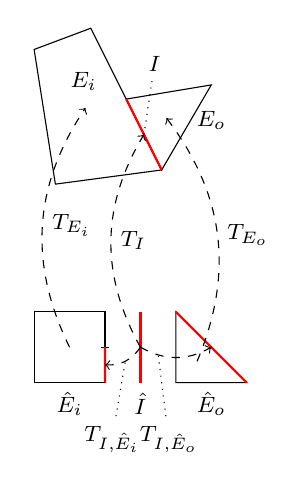
\begin{tikzpicture}[font=\footnotesize,scale=0.9]
\draw(2,0) -- (3,0) -- (2,1) -- cycle;

\draw[thick,red] (1.5,0) -- (1.5,1);

\draw (0,0) rectangle (1,1);

\draw (1.8,3) -- (1.3,4) -- (2.5,4.2) -- cycle;
\draw (1.8,3) -- (0.8,5) -- (0,4.7) -- (0.3,2.8) -- cycle;
\draw (0.95,0.5) -- (1.05,0.5);

\draw[thick,red]
  (1,0) -- (1,0.5)
  (2,1) -- (3,0)
  (1.8,3) -- (1.3,4);


\path
  (0.5,0.5) coordinate(e1r)
  (2.3,0.3) coordinate(e2r)
  (1.5,0.5) coordinate(ir)
  (0.725,3.875) coordinate(e1w)
  (1.867,3.733) coordinate(e2w)
  (1.55,3.5) coordinate(iw)
  (1,0.25) coordinate(ie1)
  (2.5,0.5) coordinate(ie2);

\draw[dashed]
  (ir)  edge[->,bend left]  node[right] {$T_I$}       (iw)
  (e1r) edge[->,bend left]  node[right] {$T_{E_i}$}   (e1w)
  (e2r) edge[->,bend right] node[right]  {$T_{E_o}$}   (e2w)
  (ir)  edge[->,bend left]  coordinate(ie1c)  (ie1)
  (ir)  edge[->,bend right] node(ie2c) [near start] {}  (ie2);

\node (ie1label) at(1.1,-0.8) {$T_{I,\hat{E}_i}$};
\node (ie2label) at(1.9,-0.8) {$T_{I,\hat{E}_o}$};
\node (ilabel) at (1.7,4.5) {$I$};

\draw[dotted]
  (ie1label) edge (ie1c)
  (ie2label) edge (ie2c.center)
  (ilabel) edge (iw);

\node at(1.5,-0.3) {$\hat{I}$};
\node at(0.5,-0.3) {$\hat{E}_i$};
\node at(2.5,-0.3) {$\hat{E}_o$};
\node at(0.7,4.25) {$E_i$};
\node at(2.5,3.7) {$E_o$};
        \end{tikzpicture}
      \end{center}
    \end{column}
  \end{columns}

\end{frame}



\begin{frame}[fragile] \frametitle{Example: Iterating over intersections}
In order to iterate over the intersections of a given grid cell with respect to some
\cpp!GridView!, use a range-based for loop with the argument \cpp!intersections(gv,cell)!.\\[.5em]
The following code iterates over all cells in a \cpp!GridView! and over all intersections of each cell:
  \begin{cppcode}
for (const auto& cell : elements(gv))
  for (const auto& is : intersections(gv,cell)) {
    if (is.boundary()) {
      // handle potential Neumann boundary
    }
    if (is.neighbor()) {
      // code for Discontinuous Galerkin or Finite Volume
    }
  }
  \end{cppcode}
\end{frame}

% \begin{frame} \frametitle{Example II}
%   \lstinputlisting[basicstyle=\scriptsize\ttfamily]{src_samples/dune_grid/intersection2.cc}
% \end{frame}

% \only<presentation>{
% \begin{frame}

%       \begin{center}

%         \vfill \vfill \vfill

%         \parbox{0.4\linewidth}{ \huge Coffee break?!  }
%         \parbox{0.3\linewidth}{
%           \includegraphics[width=\linewidth]{figures/coffee}
%         }

%         \vfill \vfill \vfill

% %        \footnotesize Dune Mug for sale at registration desk
%       \end{center}
% \end{frame}
% }

\section{Attaching Data to the Grid}
\begin{frame} \frametitle{Attaching Data to the Grid}

  For computations we need to associate data with grid entities:

  \begin{onlyenv}<1>
  \begin{itemize}
  \item spatially varying parameters,
  \item entries in the solution vector or the stiffness matrix,
  \item polynomial degree for $p$-adaptivity
  \item status information during assembling
  \item \ldots
  \end{itemize}
  \end{onlyenv}

  \begin{onlyenv}<2>
  \begin{itemize}
  \item Allow association of FE computations data with subsets of entities.
  \item Subsets could be ``vertices of level $l$'', ``faces of leaf
    elements'', \ldots
  \item Data should be stored in arrays for efficiency.
  \item Associate index/id with each entity.
  \end{itemize}
  \end{onlyenv}

\end{frame}

\begin{frame}
  \frametitle{Indices and Ids}

  \structure{Index Set:}
  provides a map $m : E \to \mathbb{N}_0$,
  where $E$ is a subset of the entities of a grid view.

  We define the subsets $E_g^c$ of a grid view
  \[ E_g^c = \{e\in E \ | \ \textrm{$e$ has codimension $c$ and geometry type $g$} \}.\]

  \begin{itemize}
  \item unique within the subsets $E_g^c$.
  \item consecutive and zero-starting within the subsets $E_g^c$.
  \item distinct leaf and a level index.
  \end{itemize}

  \pause
  \only<presentation>{\vfill}
  \structure{Id Set:}
  provides a map $m : E \to \mathbb{I}$, where $\mathbb{I}$ is a discrete
  set of ids.

  \begin{itemize}
  \item unique within $E$.
  \item ids need not to be consecutive nor positive.
  \item persistent with respect to grid modifications.
  \end{itemize}

\end{frame}

\begin{frame}[fragile]
  \frametitle{Example: Store the lengths of all edges}
  The following example demonstrates how to
  \begin{itemize}
  \item query an index set for the number of contained
    entities of a certain codimension (so that we can allocate a vector of correct size).
  \item obtain the index of a grid entity from an index set and use it to store associated data.
  \end{itemize}
  \begin{cppcode}
    auto& index_set = gv.indexSet();
    // Create a vector with one entry for each edge
    auto edge_lengths = std::vector<double>(gv.indexSet().size(1));
    // Loop over all edges and store their length
    for (const auto& edge : edges(gv))
      lengths[index_set.index(edge)] = edge.geometry().volume();
  \end{cppcode}
\end{frame}

\begin{frame}
  \frametitle{Example}
  \framesubtitle{2D Multi-Element Grid -- Indices}

  \begin{onlyenv}<presentation>
    \structure{Locally refined grid:}
    \vspace*{2ex}
    \begin{overlayarea}{\linewidth}{3ex}
      \medskip
      \begin{onlyenv}<3-6> \emph{Indices:}
      \end{onlyenv}
      \begin{onlyenv}<7-> \emph{Ids:}
      \end{onlyenv}
    \end{overlayarea}
  \end{onlyenv}

  \only<article>{\begin{multicols}{2}}
  \begin{overlayarea}{\linewidth}{0.45\linewidth}
    \begin{center}

    \begin{onlyenv}<1-2>
      \includegraphics[width=0.4\linewidth]{index-grid0}
      \hfill
      \begin{onlyenv}<2>
        \includegraphics[width=0.4\linewidth]{index-grid1}\par
        \only<article>{Locally refined grid\par}
      \end{onlyenv}
    \end{onlyenv}

    \begin{onlyenv}<3>
      \includegraphics[width=0.4\linewidth]{index-vertex0}
      \hfill
      \includegraphics[width=0.4\linewidth]{index-grid1}\par
      Consecutive index for vertices\par
    \end{onlyenv}

    \begin{onlyenv}<4>
      \includegraphics[width=0.4\linewidth]{index-all0}
      \hfill
      \includegraphics[width=0.4\linewidth]{index-grid1}\par
      \ldots{} and cells\par
    \end{onlyenv}

    \begin{onlyenv}<5>
      \includegraphics[width=0.4\linewidth]{index-cell0}
      \hfill
      \includegraphics[width=0.4\linewidth]{index-cell1old}\par
      Old cell indices on refined grid\par
    \end{onlyenv}

    \begin{onlyenv}<6>
      \includegraphics[width=0.4\linewidth]{index-cell0}
      \hfill
      \includegraphics[width=0.4\linewidth]{index-cell1}\par
      Consecutive cell indices on coarse and refined grid\par
    \end{onlyenv}

    \begin{onlyenv}<7>
      \includegraphics[width=0.4\linewidth]{index-id0}
      \hfill
      \includegraphics[width=0.4\linewidth]{index-id1}\par
      Persistent Ids on coarse and refined grid\par
    \end{onlyenv}

    \end{center}
  \end{overlayarea}
  \only<article>{\end{multicols}}
\end{frame}

\begin{frame} \frametitle{Mapper}
  Mappers extend the functionality of Index Sets.

  \begin{itemize}
  \item associate data with an arbitrary subsets $E'\subseteq E$
    \only<presentation>{\\}
    of the entities $E$ of a grid.
  \item the data $D(E')$ associated with
    $E'$ is stored in an array.
  \item map from the consecutive, zero-starting index $I_{E'} =
    \{0, \ldots, |E'|-1\}$ to the data set $D(E')$.
  \end{itemize}

  Mappers can be easily implemented upon the Index Sets and Id Sets.

  You will be using the
  \footnotesize
  \cpp!Dune::MultipleCodimMultipleGeomTypeMapper<GridView,Layout>!.
\end{frame}

 \only<article>{\newpage}

\begin{frame} \frametitle{Example}
\scriptsize
\begin{codeblock}
\inputminted[lastline=20]{c++}{src_samples/dune_grid/indizes_cxx11.cc}
\end{codeblock}
  % \only<presentation>{
  %   \lstinputlisting[lastline=20, basicstyle=\scriptsize\ttfamily]{src_samples/dune_grid/indizes_cxx11.cc}
  % }
  % \only<article>{
  %   \lstinputlisting[basicstyle=\scriptsize\ttfamily]{src_samples/dune_grid/indizes_cxx11.cc}
  % }
\end{frame}

\begin{onlyenv}<presentation>
\begin{frame} \frametitle{Example II}
\scriptsize
\begin{codeblock}
\inputminted[firstline=17]{c++}{src_samples/dune_grid/indizes_cxx11.cc}
\end{codeblock}
\end{frame}
\end{onlyenv}

\begin{onlyenv}<presentation>
  \begin{frame}
    \frametitle{Further Topics}
    \only<presentation>{\framesubtitle{What we didn't discuss\dots{}}}
    \begin{itemize}
    \item Grid Adaptation
    \item Parallelization
    \item IO
    \item More specialized methods
    \end{itemize}
  \end{frame}
\end{onlyenv}

\section{Further Reading}
\begin{frame} \frametitle<presentation>{Further Reading}
  \begin{thebibliography}{}

\bibitem[Bastian et al. (2008)]{dune01}
P. Bastian, M. Blatt, A. Dedner, C. Engwer, R. Klöfkorn, M. Ohlberger,
O. Sander.
\newblock A Generic Grid Interface for Parallel and Adaptive
Scientific Computing.
\emph{Part I: Abstract Framework.}
\newblock \emph{Computing,} 82(2--3), 2008, pp.~103--119.

\bibitem[Bastian et al. (2008)]{dune02}
P. Bastian, M. Blatt, A. Dedner, C. Engwer, R. Klöfkorn, M. Ohlberger,
O. Sander.
\newblock A Generic Grid Interface for Parallel and Adaptive
Scientific Computing.
\emph{Part II: Implementation and Tests in DUNE.}
\newblock \emph{Computing,} 82(2--3), 2008, pp.~121--138.

\end{thebibliography}
\end{frame}

\end{document}
